\def \path {misc/dtcwt_gain}
\def \imgpath {\path/images}

\section{Introduction}\label{sec:intro}

Using wavelet based methods with deep learning is nascent but not novel.
Wavelets have been applied to texture classification \cite{fujieda_wavelet_2017,
sifre_combined_2012}, super-resolution \cite{guo_deep_2017} and for adding
detail back into dense pixel-wise segmentation tasks \cite{ma_detailed_2018}.
One exciting piece of work built on wavelets is the Scattering Transform
\cite{mallat_group_2012}, which has been used as a feature extractor for
learning, firstly with simple classifiers \cite{bruna_invariant_2013,
singh_scatternet_2017}, and later as a front end to hybrid deep learning
tasks\cite{oyallon_scaling_2017, singh_scatternet_2018}. Despite their power and
simplicity, scattering features are fixed and are visibly different to regular
CNN features \cite{cotter_visualizing_2017} - their nice invariance properties
come at the cost of flexibility, as there is no ability to learn in between
scattering layers. 

For this reason, we have been investigating a slightly different approach, more
similar to the Fourier based work in \cite{rippel_spectral_2015} in which Rippel
et.\ al.\ investigate parameterization of filters in the Fourier domain. In the
forward pass, they take the inverse DFT of their filter, and then apply normal
pixel-wise convolution. We wish to extend this by not only parameterizing
filters in the wavelet domain, but by performing the convolution there as well
(i.e., also taking the activations into the wavelet domain). After processing is
done, we can return to the pixel domain. Doing these forward and inverse
transforms has two significant advantages: 

\begin{enumerate}
  \item The layers can easily replace standard convolutional layers if they
    accept and return the same format.
  \item We can learn both in the wavelet and pixel space.
\end{enumerate}

As neural network training involves presenting thousands of training samples, we
want our layer to be fast. To achieve this we would ideally choose to use a
critically sampled filter bank implementation. The fast 2-D Discrete Wavelet
Transform (DWT) is a possible option, but it has two drawbacks: it has poor
directional selectivity and any alteration of wavelet coefficients will cause
the aliasing cancelling properties of the reconstructed signal to disappear.
Instead we choose to use the Dual-Tree Complex Wavelet Transform (\DTCWT)
\cite{selesnick_dual-tree_2005} as at the expense of limited redundancy (4:1),
it enables us to have better directional selectivity, and allows us to modify
the wavelet coefficients and still have minimal aliasing terms when we
reconstruct \cite{kingsbury_complex_2001}.

\Autoref{sec:method} of the paper describes the implementation details of our design, and
\autoref{sec:results} describes the experiments and results we have done so far.

\section{Similar Work}
\subsection{Parameterizing filters in Fourier Domain}
\cite{rippel_spectral_2015} explored parameterization of filters in the DFT
domain.  Note that they do not necessarily do the convolution in the Frequency
domain, they simply parameterize a filter $\vec{w} \in \reals[F\x C\x K\x K]$ as
a set of fourier coefficients $\hat{\vec{w}} \in \complexes[F\x C\x K \x \ceil{K/2}]$
(the reduced spatial size is a result of enforcing that the inverse DFT of their
filter to be real, so the parameterization is symmetric). On the forward pass of
the neural network, they take the inverse DFT of $\hat{\vec{w}}$ to obtain
$\vec{w}$ and then convolve this with the input $\vec{x}$ as a normal CNN
would do.\footnote{The convolution may be done by taking both the image and
filter back into the fourier space but this is typically decided by the
framework, which selects the optimal convolution strategy for the filter and
input size. Note that there is not necessarily a saving to be gained by
enforcing it to do convolution by product of FFTs, as the FFT size needed for
the filter will likely be larger than $K\x K$, which would require resampling
the coefficients}.

Note that this is almost identical to a normal CNN, except it allows for
slightly a reworked filter initialization and regularization, as well as 
affecting optimizers that keep track of past updates (such as SGD with momentum, 
Adam \cite{kingma_adam:_2014} or Adagrad). \autoref{fig:rippel_spectral_figs}
shows the fourier and spatial representation of some of the filters in
\cite{rippel_spectral_2015}, as well as histograms showing the sparsity of
parameters and momenta for parameter updates. The lower mean in the distribution
of parameter momenta indicates that fewer parameters are being updated in a
constant direction.

\subsubsection{Initialization}
No specific mention is made of the initialization technique used but it may well
be helpful to put a prior over the spectra.

\subsubsection{Regularization}
Due to Parseval's theorem, it is clear that applying an L2 regularization on the
filter weights :

$$\sum_i \lnorm{w_i}{2}^2 = \sum_i \lnorm{\hat{w}_i}{2}^2 = \sum_i
  \lnorm{\real{\hat{w_i}}}{2}^2 + \lnorm{\imag{\hat{w_i}}}{2}^2 $$

However can apply L1 regularization on the complex magnitude of the DFT filter
weights to impose spectral sparsity.

\subsubsection{Optimization}
If we define the DFT as the orthonormal version, i.e. for a square image, let:

$$ U_{ab} = \frac{1}{\sqrt{N}} \exp\{ \frac{-2j\pi ab}{N} \} $$

then

\begin{align}
  Y &= \F{DFT}\{ X \} = UXU \\
  X &= \F{DFT}^{-1} \{ Y \} = U^*YU^* \\
  \Delta X &= \dydx{L}{X} = U^* \Delta Y U^* = \F{DFT}^{-1} \{\Delta Y \}\\
  \Delta Y &= \dydx{L}{Y} = U \Delta X U = \F{DFT} \{\Delta X \}
\end{align}

Parameterizing in the fourier domain does not affect linear optimizers like
vanilla SGD and SGD with momentum (including with Nesterov momentum). 
For example consider a single filter
parameterized in the DFT and spatial domains presented with the exact same data
(and for the moment with no regularization). Let the initial values for 
$\hat{\vec{w}}$ and $\vec{w}$ be:

\begin{align}
  \hat{\vec{w}}_1 &= \alpha \\
  \vec{w}_1 &= \beta = \F{DFT}^{-1}\{\alpha\} 
\end{align}

After presenting both systems with the same minibatch of samples $\mathcal{D}$
and calculating the gradient $\dydx{L}{\vec{w}}$ we update both parameters:

\begin{eqnarray*}
  \vec{w}_2 & = & \vec{w}_1 - \eta \left. \dydx{L}{\vec{w}} \right|_{\vec{w} = \beta} \\
            & = & \beta - \eta \delta_{\vec{w}}  \\
  \hat{\vec{w}}_2 & = & \hat{\vec{w}}_1 - \eta \left. \dydx{L}{\hat{\vec{w}}} \right|_{ \hat{\vec{w}} = \alpha}  \\
                  & = & \alpha - \eta \F{DFT} \{ \delta_{\vec{w}} \} 
\end{eqnarray*}

We can then compare the effect the new parameters would have on the next
minibatch by calculating $\F{DFT}^{-1} \{\hat{\vec{w}}_2 \}$:
\begin{eqnarray*}
  \F{DFT} ^{-1} \{ \hat{\vec{w}}_2 \} &=& \F{DFT} ^{-1} \left\{ \alpha - \eta \F{DFT} \{ \delta_{\vec{w}} \} \right\}  \\
       & = & \F{DFT}^{-1} \left \{ \alpha \right \} - \eta \F{DFT}^{-1} \left \{ \F{DFT} \{ \delta_{\vec{w}} \} \right \} \\
       & = & \beta - \eta \delta_{\vec{w}} \\
       & = & \vec{w}_2
\end{eqnarray*}

In fact it can easily be seen that any optimizer that uses linear combinations
of gradients makes this new parameterization identical to parameterization in
the spatial domain. Optimizers like Adam and Adagrad however have update rules
that are not simply linear combinations of past gradients and so this affects
the learning trajectory. For Adam, there is a step where the gradients are
squared to estimate the variance of the parameter updates. 

This shows that any work involving reparametrizing or rethinking filter
convolution must be careful in what is done.

Further to this, while the inspiration for the work comes from wanting to remain
in the frequency domain, it is unsatisfying to simply parameterize filters there
and then take the inverse DFT and perform normal convolution. Ideally we would
like to fully take advantage of the benefits of a frequency representation.

\begin{figure}
  \centering
  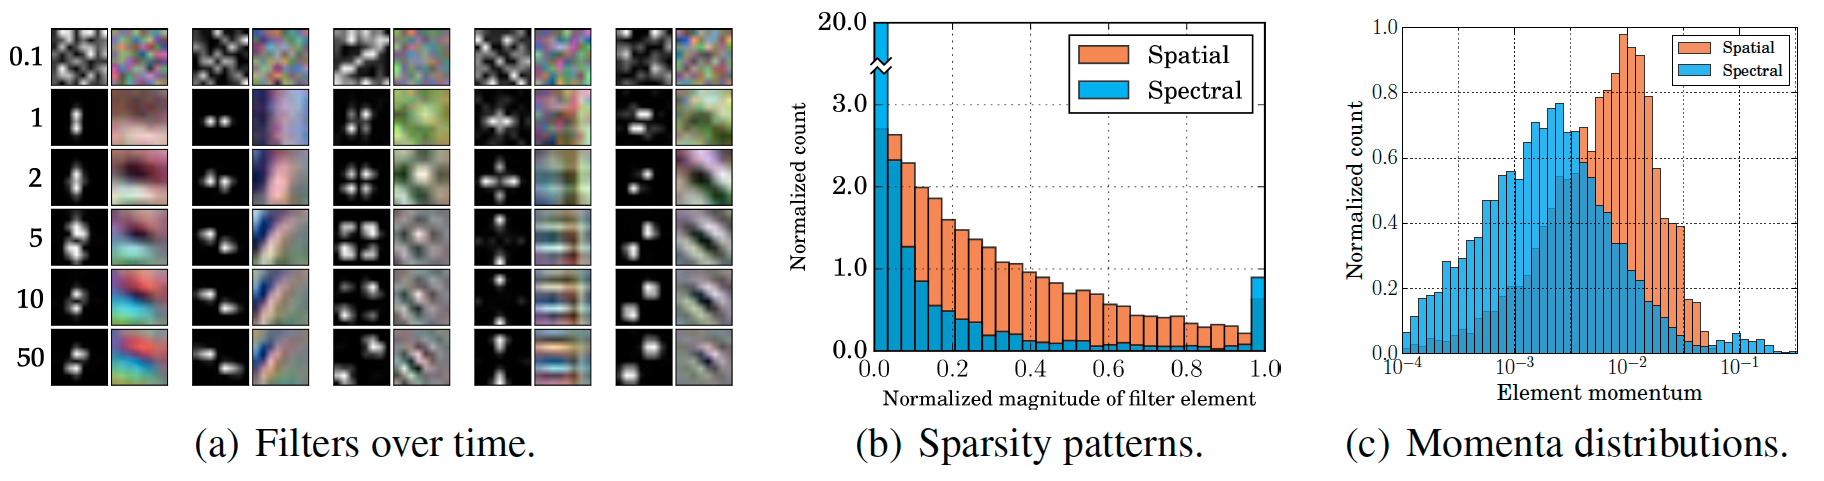
\includegraphics[width=\textwidth]{\imgpath/rippel.png}
  \mycaption{Learning Dynamics of CNNs with DFT parameterization}{(a)
  Progression over several epochs of filters parametrized in the frequency
  domain. The left column shows the parameterized filter and the right column
  its inverse DFT. (b) Sparsity patterns for different parameterizations -
  spectral representations tend to be sparser. (c) Momenta distributions for
  parameters of CNNs trained with and without spectral parameterization. In the
  spectral parameterization fewer parameters are updated.  Image taken from
  \cite{rippel_spectral_2015}.}
  \label{fig:rippel_spectral_figs}
\end{figure}


\subsection{Spectral Pooling}
The Spectral Pooling method introduced in \cite{rippel_spectral_2015} is
described in the paper as:

\begin{quote}
  We assume we are given an input $\vec{x}\in \reals[M\x N]$, and some desired
  output map dimensionality $H \x W$. First we compute the discrete Fourier
  transform of the input into the frequency domain as $y = \mathcal{F}(\vec{x})
  \in \complexes[M\x N]$, and assume that the DC componenet has been shifted to
  the center of the domain as is standard practice. We then crop the frequency
  representation by maintaining only the central $H\x W$ submatrix of
  frequencies, which we denote as $\hat{\vec{y}} \in \complexes[H\x W]$. Finally, we
  map this approximation back into the spatial domain by taking its inverse DFT
  as $\hat{\vec{x}} = \mathcal{F}^{-1}(\hat{\vec{y}}) \in \reals[H\x W]$.
\end{quote}

While they have chosen to do this in the Fourier domain, this could also be
achieved by convolving with a separable, resampled 2D sinc function of the
appropriate frequencies for the horizontal and vertical directions:

$$\hat{\vec{x}} = \frac{HW}{MN} \vec{x} \conv \F{sinc}(\frac{Hn_y}{M}) \conv
\F{sinc}(\frac{Wn_x}{N})$$

where $n_x \in \{??\}, n_y \in \{??\}$. Of course, sincs have infinite support
in the time domain, so to achieve a similar result to spectral pooling you would
have to convolve with windowed sincs, or do some other form of similar low pass
filtering with resampling. In \cite{williams_wavelet_2018} they do exactly this
and call it `wavelet pooling', which is just keeping the low-low output of a
separable 2D DWT, or simply convolving with a separable lowpass filter. They
experimentally showed that this was equivalent to spectral and average pooling.

Note that speed ups could be achieved here if the convolution is done in the
Fourier domain, as it would involve only computing the reduced spectrum size
before taking inverse DFTs.


\section{Aliasing in the DWT}
Consider a single level critically sampled DWT in 1-D. The aliasing cancelling
condition is:

$$G_0(z)H_0(-z) + G_1(z)H_1(-z) = 0$$

This is typically solved by using Quadrature Mirror Filters, i.e.

\begin{align}
  H_1(z) &= H_0(-z) \\
  G_0(z) &= H_0(z) \\
  G_1(z) &= -H_1(z) = -H_0(-z) 
\end{align}

\section{Shift Invariance of the \DTCWT}

\begin{figure}
  \centering
  \begin{tikzpicture}
    \matrix (m1) [minimum height=4mm, column sep=6mm, align=center]
	{
	%--------------------------------------------------------------------
		\node[coordinate]                  (m00) {};    &
		\node[coordinate]                  (m01) {};          &
		\node[dspsquare]                   (m02) {$A(z)$};          &
		\node[circle,draw,inner sep=1pt]   (m03) {\downsamplertext{M}}; &
		\node[dspnodeopen,dsp/label=above] (m04) {$X_a(z)$};          &
		\node[circle,draw,inner sep=1pt]   (m07) {\upsamplertext{M}}; &
		\node[dspsquare]                   (m08) {$C(z)$};          &
		\node[coordinate]                  (m09) {};          &
		\node[coordinate]                  (m0X) {};          \\
		%--------------------------------------------------------------------
		\node[dspnodefull]                 (m10) {};          &
		\node[coordinate]                  (m11) {};          &
		\node[coordinate]                  (m12) {};    &
		\node[coordinate]                  (m13) {};          &
		\node[coordinate]                  (m14) {};    &
		\node[coordinate]                  (m17) {};          &
		\node[coordinate]                  (m18) {};    &
		\node[dspadder]                    (m19) {};          &
		\node[]     (m1X) {};          \\
		%--------------------------------------------------------------------
		\node[coordinate]                  (m20) {};    &
		\node[coordinate]                  (m21) {};          &
		\node[dspsquare]                   (m22) {$B(z)$};          &
		\node[circle,draw,inner sep=1pt]   (m23) {\downsamplertext{M}}; &
		\node[dspnodeopen,dsp/label=below] (m24) {$X_b(z)$};          &
		\node[circle,draw,inner sep=1pt]   (m27) {\upsamplertext{M}}; &
		\node[dspsquare]                   (m28) {$D(z)$};          &
		\node[coordinate]                  (m29) {};          &
		\node[coordinate]                  (m2X) {};          \\
		%--------------------------------------------------------------------
	};
	\draw[dspline] (m10) -- (m11);
	\draw[dspline] (m11) -- (m01);
	\draw[dspline] (m11) -- (m21);
	\foreach \i in {0,2} {
    	\draw[dspconn] (m\i1) -- (m\i2);
    	\draw[dspconn] (m\i2) -- (m\i3);
    	\draw[dspline] (m\i3) -- (m\i4);
    	\draw[dspconn] (m\i4) -- (m\i7);
    	\draw[dspconn] (m\i7) -- (m\i8);
    	\draw[dspline] (m\i8) -- (m\i9);
	}
  \node[left=0pt of m10] (left) {$X(z)$};
  \node[below=9pt of m24] (bottom) {};
  \draw[dspconn] (m09) -- node[right, yshift=5pt] {$Y_a(z)$} (m19);
  \draw[dspconn] (m29) -- node[right, yshift=-5pt] {$Y_b(z)$} (m19);
  \draw[dspconn] (m19) -- node[right, xshift=5pt] {$Y(z)$} (m1X);
	
\end{tikzpicture}

  \mycaption{Block Diagram of 1-D \DTCWT}{Note the top and bottom paths are
  through the wavelet or scaling functions from just level m ($M=2^m$). Figure
  based on Figure~4 in \cite{kingsbury_complex_2001}.}
  \label{fig:dtcwt_two_tree}
\end{figure}

\autoref{fig:dtcwt_two_tree} shows the path through the two trees for one band
of the full tree. We ignore the other paths through the tree for the moment 
(e.g. consider setting all the coefficients to 0). 

The output from \autoref{fig:dtcwt_two_tree} is:

$$ Y(z) = Y_a(z) + Y_b(z) = \frac{1}{M}\sum_{k=0}^{M-1} X\left(W^k z\right)
  \left[ A\left(W^kz\right)C(z) + B\left(W^kz\right)D(z) \right] $$

Where $W=e^{j2\pi/M}$.  To achieve shift invariance we need 
$A\left(W^kz\right)C(z) + B\left(W^kz\right)D(z)$ to be very small or to cancel
each other out for all $k \neq 0$.

The complex analysis filter (taking us into the wavelet domain) is 

$$P(z) = \frac{1}{2}\left(A(z)+jB(z)\right)$$

and the complex synthesis filter (returning us to the pixel domain) is 

$$Q(z) = \frac{1}{2}\left(C(z) - jD(z)\right)$$

where $A,B,C,D$ are real.  If $G(z) = G_r(z) + jG_i(z) = 1$ then the end-to-end
transfer function is (from section 4 of \cite{kingsbury_complex_2001}):

\begin{equation}\label{eq:end_to_end1}
\frac{Y(z)}{X(z)} = \frac{2}{M}\left(P(z)Q(z) + P^*(z)Q^*(z)\right)
\end{equation}

where $P, Q$ have support only in the top half of the Fourier plane and $P^*,
Q^*$ are $P$ and $Q$ reflected in the horizontal frequency axis. Examples of
$P(z)Q(z)$ for different subbands of a 2-D \DTCWT have spectra shown in
\autoref{fig:dtcwt_bands_freq}, $P^*(z)Q^*(z)$ make up the missing half of the
frequency space.\\

\section{Method}\label{sec:method}

\begin{figure}[ht]
  \centering
  \subfloat[]{%
    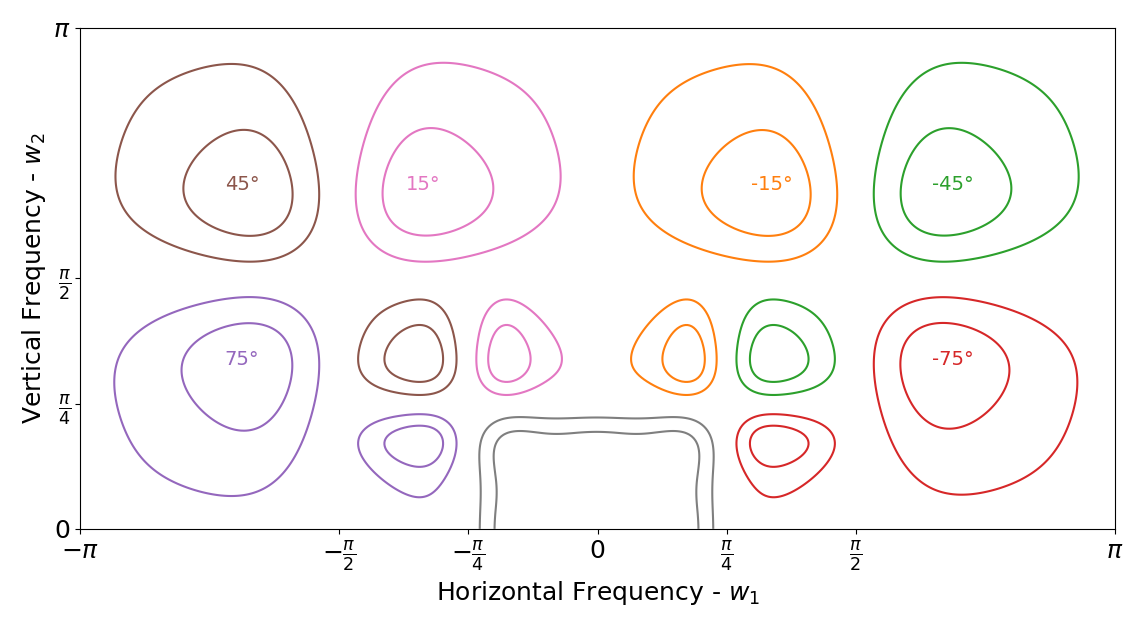
\includegraphics[height=6cm]{\imgpath/subbands.png}
    \label{fig:dtcwt_bands_freq}
  }
  \hspace{1cm}
%    \newline
  \subfloat[]{%
    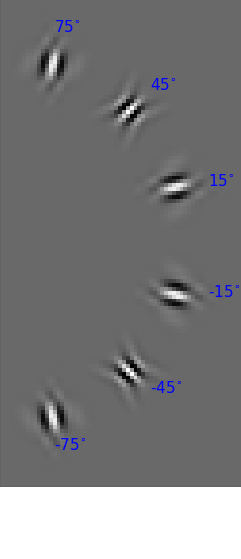
\includegraphics[height=5.7cm]{\imgpath/impulses.png}
    \label{fig:dtcwt_bands_impulse}
  }
  \newline
  \subfloat[]{%
    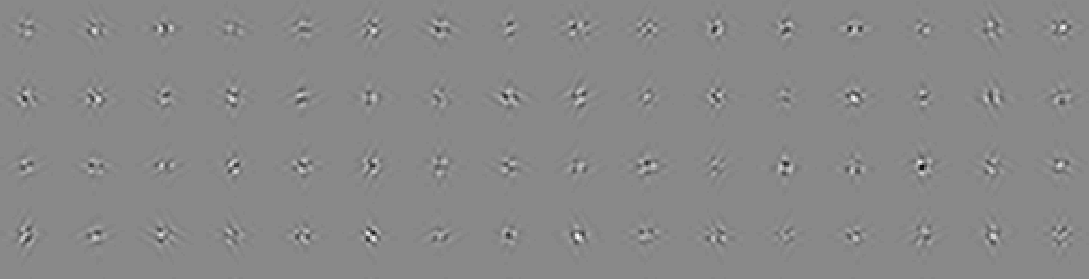
\includegraphics[width=.8\textwidth]{\imgpath/examples_scale2.png}
    \label{fig:example_impulses}
  }
  \mycaption{Building blocks of the \DTCWT gain
    layer}{\subref{fig:dtcwt_bands_freq} Contour plots at -1dB and -3dB showing the
    support in the Fourier domain of the 6 subbands of the \DTCWT at scales 1
    and 2 and the scale 2 lowpass. These are the product $P(z)Q(z)$ from
    \autoref{eq:end_to_end1}.% \subref{fig:dtcwt_bands_impulse} The pixel domain
    impulse responses for the second scale wavelets.
    \subref{fig:example_impulses} Example impulses of our layer when $g_1$, and
    $g_{lp}$ are 0 and $g_2 \in \mathbb{C}^{6\x 1\x 1}$, with each real and
    imaginary element drawn from $\mathcal{N}(0,1)$. I.e., only information in
    the 6 subbands with $\frac{\pi}{4} < |w_1|, |w_2| < \frac{\pi}{2}$ from
    \subref{fig:dtcwt_bands_freq} is passed through.} 
  \label{fig:dtcwt_bands}
\end{figure}

In a standard convolutional layer, an input with $C$ channels, $H$ rows and $W$
columns is $X \in \reals[C\x H\x W]$, which is then convolved with $F$ filters
of spatial size $K$ - $w \in \reals[F \x C\x K\x K]$, giving $Y \in \reals[F\x
H\x W]$. In many systems like \cite{krizhevsky_imagenet_2012, he_deep_2015}, the
first layer is typically a selection of bandpass filters, selecting edges with
different orientations and center frequencies. In the wavelet space this would
be trivial - take a decomposition of each input channel and keep individual
subbands (or equivalently, attenuate other bands), then take the inverse wavelet
transform.  \autoref{fig:dtcwt_bands} shows the frequency space for the \DTCWT
and makes it clearer as to how this could be done practically for a two scale
transform. To attenuate all but say the $15 \degs$ band at the first scale for
the first input channel, we would need to have $13C$ gains for the 13 subbands
and $C$ input channels, $13C-1$ of which would be zero and the remaining
coefficient one.

Instead of explicitly setting the gains, we can randomly initialize them and use
backpropagation to learn what they should be. This gives us the power to learn
more complex shapes rather than simple edges, as we can mix the regions of the
frequency space per input channel in an arbitrary way. 

\subsection{Memory Cost}

Again considering a two scale transform --- instead of learning $w\in \reals[F
\x C\x K\x K]$ we learn complex gains at the two scales, and a real gain for the
real lowpass:

$$
\begin{align}
  g_1 & \in & \complexes[F\x C\x 6\x 1\x 1] \\
  g_2 &\in &\complexes[F\x C\x 6\x 1\x 1] \\
  g_{lp} &\in & \reals[F\x C\x 1\x 1]
\end{align}
$$

We have set the spatial dimension to be $1\x 1$ to show that this gain is
identical to a $1\x 1$ convolution over the complex wavelet coefficients. If we
wish, we can learn larger spatial sizes to have more complex
attenuation/magnification of the subbands. We also can use more/fewer than
2 wavelet scales.  At first glance, we have increased our parameterization by
  a factor of 25 (13 subbands, of which all but the lowpass are complex), but
each one of these gains affects a large spatial size. For the first scale, the
effective size is about $5\x 5$ pixels, for the second scale it is about $15\x
15$.

\begin{figure}[]
  \centering
  \makebox[\textwidth][c]{%
    \resizebox{1.1\textwidth}{!}{\begin{tikzpicture}
    \matrix (m1) [row sep=5mm, column sep=6mm,align=center,anchor=center]
	{
	% %--------------------------------------------------------------------
		% \node[coordinate]                  (m00) {};    &
		% \node[coordinate]                  (m01) {};          &
		% \node[dspsquare]                   (m02) {$A(z)$};          &
		% \node[circle,draw,inner sep=1pt]   (m03) {\downsamplertext{M}}; &
		% \node[dspnodeopen,dsp/label=above] (m04) {$V_r(z)$};          &
		% \node[rectangle,draw,inner sep=2pt](m05) {$G_r(z)$}; &
		% \node[dspnodeopen,dsp/label=above] (m06) {$W_r(z)$};          &
		% \node[circle,draw,inner sep=1pt]   (m07) {\upsamplertext{M}}; &
		% \node[dspsquare]                   (m08) {$C(z)$};          &
		% \node[coordinate]                  (m09) {};          &
		% \node[coordinate]                  (m0X) {};          \\
		% %--------------------------------------------------------------------
		% \node[]                            (m10) {$X(z)$};          &
		% \node[coordinate]                  (m11) {};          &
		% \node[coordinate]                  (m12) {};    &
		% \node[coordinate]                  (m13) {};          &
		% \node[coordinate]                  (m14) {};    &
		% \node[coordinate]                  (m15) {};          &
		% \node[coordinate]                  (m16) {};    &
		% \node[coordinate]                  (m17) {};          &
		% \node[coordinate]                  (m18) {};    &
		% \node[dspadder]                    (m19) {};          &
    % \node[]                            (m1X) {$Y(z)$};          \\
		% %--------------------------------------------------------------------
		% \node[coordinate]                  (m20) {};    &
		% \node[coordinate]                  (m21) {};          &
		% \node[dspsquare]                   (m22) {$B(z)$};          &
		% \node[circle,draw,inner sep=1pt]   (m23) {\downsamplertext{M}}; &
		% \node[dspnodeopen,dsp/label=below] (m24) {$V_i(z)$};          &
		% \node[rectangle,draw,inner sep=2pt](m25) {$G_r(z)$}; &
		% \node[dspnodeopen,dsp/label=below] (m26) {$W_i(z)$};          &
		% \node[circle,draw,inner sep=1pt]   (m27) {\upsamplertext{M}}; &
		% \node[dspsquare]                   (m28) {$D(z)$};          &
		% \node[coordinate]                  (m29) {};          &
		% \node[coordinate]                  (m2X) {};          \\
		% %--------------------------------------------------------------------
		% &&&&&&&&& \\
		\node[coordinate]                  (m00a) {};    &
		\node[coordinate]                  (m01a) {};          &
		\node[dspsquare]                   (m02a) {$A\left(z^{-1}\right)$};          &
		\node[circle,draw,inner sep=1pt]   (m03a) {\upsamplertext{M}}; &
		\node[dspnodeopen,dsp/label=above] (m04a) {$\Delta U_r(z)$};          &
		%\node[coordinate]                  (m05) {}; &
		\node[rectangle,draw,inner sep=2pt](m05a) {$G_r\left(z^{-1}\right)$}; &
		\node[dspnodeopen,dsp/label=above] (m06a) {$\Delta V_r(z)$};          &
		\node[circle,draw,inner sep=1pt]   (m07a) {\downsamplertext{M}}; &
		\node[dspsquare]                   (m08a) {$C\left(z^{-1}\right)$};          &
		\node[coordinate]                  (m09a) {};          &
		\node[coordinate]                  (m0Xa) {};          \\
		%--------------------------------------------------------------------
		%\node[coordinate]  (m10) {$\Delta X(z)$};          &
    \node[]                            (m10a) {$\Delta X(z)$}; &
		\node[dspadder]                    (m11a) {};          &
		\node[coordinate]                  (m12a) {};    &
		\node[coordinate]                  (m13a) {};          &
		\node[coordinate]                  (m14a) {};    &
		\node[coordinate]                  (m15a) {};          &
		\node[coordinate]                  (m16a) {};    &
		\node[coordinate]                  (m17a) {};          &
		\node[coordinate]                  (m18a) {};    &
		\node[coordinate]                  (m19a) {};          &
		\node[]                            (m1Xa) {$\Delta Y(z)$};          \\
		%--------------------------------------------------------------------
		\node[coordinate]                  (m20a) {};    &
		\node[coordinate]                  (m21a) {};          &
		\node[dspsquare]                   (m22a) {$B\left(z^{-1}\right)$};          &
		\node[circle,draw,inner sep=1pt]   (m23a) {\upsamplertext{M}}; &
		\node[dspnodeopen,dsp/label=below] (m24a) {$\Delta U_i(z)$};          &
		%\node[coordinate]                  (m25) {}; &
		\node[rectangle,draw,inner sep=2pt](m25a) {$G_r\left(z^{-1}\right)$}; &
		\node[dspnodeopen,dsp/label=below] (m26a) {$\Delta V_i(z)$};          &
		\node[circle,draw,inner sep=1pt]   (m27a) {\downsamplertext{M}}; &
		\node[dspsquare]                   (m28a) {$D\left(z^{-1}\right)$};          &
		\node[coordinate]                  (m29a) {};          &
		\node[coordinate]                  (m2Xa) {};          \\
		%--------------------------------------------------------------------
	};
	% \draw[dspline] (m10) -- (m11);
	% \draw[dspline] (m11) -- (m01);
	% \draw[dspline] (m11) -- (m21);
	% \foreach \i in {0,2} {
      % \draw[dspconn] (m\i1) -- (m\i2);
      % \draw[dspconn] (m\i2) -- (m\i3);
      % \draw[dspline] (m\i3) -- (m\i4);
      % \draw[dspconn] (m\i4) -- (m\i5);
      % \draw[dspline] (m\i5) -- (m\i6);
      % \draw[dspconn] (m\i6) -- (m\i7);
      % \draw[dspconn] (m\i7) -- (m\i8);
      % \draw[dspline] (m\i8) -- (m\i9);
	% }
	% %\draw[dspflow] (m04) --  (m06);
	% %\draw[dspflow] (m24) -- (m26);
	% \draw[dspconn] (m24) -- node[draw,pos=0.7,inner sep=2pt,fill=white] {$-G_i(z)$} (m06);
	% \draw[dspconn] (m04) -- node[draw,pos=0.7,inner sep=2pt,fill=white] {$G_i(z)$} (m26);
	% \draw[dspconn] (m09) -- (m19);
	% \draw[dspconn] (m29) -- (m19);
	% \draw[dspconn] (m19) -- (m1X);
	\draw[dspconn] (m11a) -- (m10a);
	\draw[dspconn] (m01a) -- (m11a);
	\draw[dspconn] (m21a) -- (m11a);
	\foreach \i in {0,2} {
    	\draw[dspconn] (m\i9a) -- (m\i8a);
    	\draw[dspconn] (m\i8a) -- (m\i7a);
    	\draw[dspline] (m\i7a) -- (m\i6a);
    	\draw[dspconn] (m\i6a) -- (m\i5a);
    	\draw[dspline] (m\i5a) -- (m\i4a);
    	\draw[dspconn] (m\i4a) -- (m\i3a);
    	\draw[dspconn] (m\i3a) -- (m\i2a);
    	\draw[dspline] (m\i2a) -- (m\i1a);
	}
	%\draw[dspflow] (m04) --  (m06);
	%\draw[dspflow] (m24) -- (m26);
	\draw[dspconn] (m06a) -- node[draw,pos=0.7,inner sep=2pt,fill=white] {$-G_i\left(z^{-1}\right)$} (m24a);
	\draw[dspconn] (m26a) -- node[draw,pos=0.7,inner sep=2pt,fill=white] {$G_i\left(z^{-1}\right)$} (m04a);
	\draw[dspline] (m09a) -- (m19a);
	\draw[dspline] (m29a) -- (m19a);
	\draw[dspline] (m19a) -- (m1Xa);
	
\end{tikzpicture}
}
  }
  \mycaption{Block Diagram of 1-D \DTCWT gain layer}{(Top) 
  Forward and (bottom) backward pass of our system, based on
    Figure~4 in \cite{kingsbury_complex_2001}. Ignoring the $G$ gains, the top
    and bottom paths (through $A, C$ and $B, D$ respectively) make up the the
    real and imaginary parts for \emph{one subband} of the dual tree system.
    Combined, $A+jB$ and $C-jD$ make the complex filters necessary to have
    support on one side of the Fourier domain (see \autoref{fig:dtcwt_bands}).
    Adding in the complex gain $G_r + jG_i$, we can now attenuate/shape the
    impulse response in each of the subbands. To allow for learning, we need
    backpropagation. The bottom diagram indicates how to pass gradients $\Delta
    Y(z)$ through the layer. Note that upsampling has become downsampling, and
    convolution has become convolution with the time reverse of the filter
    (represented by $z^{-1}$ terms).}
  \label{fig:fwd_bwd}
\end{figure}

\subsection{Computational Cost}

A standard convolutional layer needs $K^2 F$ multiplies per input pixel (of
which there are $C\x H\x W$). In comparison, the wavelet gain method does a set
number of operations per pixel for the forward and inverse transforms, and then
applies gains on subsampled activations. For a 2 level \DTCWT the transform
overhead is about 60 multiplies for both the forward and inverse transform. It
is important to note that unlike the filtering operation, this does not scale
with $F$. The learned gains in each subband do scale with the number of output
channels, but can have smaller spatial size (as they have larger effective
sizes) as well as having fewer pixels to operate on (because of the decimation).
The end result is that as $F$ and $C$ grow, the overhead of the $C$ forward and
$F$ inverse transforms is outweighed by cost of $FC$ mixing processes, which
should in turn be significantly less than the cost of $FC$ $K\x K$ standard
convolutions for equivalent spatial sizes.

\subsection{Examples}

\autoref{fig:example_impulses} show example impulse responses of our layer.
These impulses were generated by randomly initializing both the real and
imaginary parts of $g_2 \in \complexes[6\x 1\x 1]$ from $\mathcal{N}(0,1)$ and
$g_1, g_{lp}$ are set to 0. I.e.\ each shape has 12 random variables. It is good
to see that there is still a large degree of variability between shapes. Our
experiments have shown that the distribution of the normalized cross-correlation
between 512 of such randomly generated shapes matches the distribution for
random vectors with roughly 11.5 degrees of freedom.

\subsection{Forward propagation}

\autoref{fig:fwd_bwd} shows the block diagram using $Z$-transforms for a single
band of our system (it is based on Figure~4 in \cite{kingsbury_complex_2001}).
To keep things simple for the rest of \autoref{sec:method} the figure shown is
for a 1-D system; it is relatively straightforward to extend this to
2-D\cite{selesnick_dual-tree_2005}. %
Modifying this from the standard wavelet equations by adding the subband gains
$G_r(z)$ and $G_i(z)$, the transfer function becomes:

\begin{equation}\label{eq:end_to_end2}
  \begin{split}
    \frac{Y(z)}{X(z)} = \frac{2}{M} \left[ \right. & G_r(z^M) \left( P(z)Q(z) + P^*(z)Q^*(z) \right) +  \\ 
     & \left. jG_i(z^M) \left(P(z)Q(z)-P^*(z)Q^*(z) \right) \right]
  \end{split}
\end{equation}

\begin{table}[]
  \centering
{\renewcommand{\arraystretch}{1.2}
  \captionsetup{width=\textwidth}
  \mycaption{LeNet vs WaveLeNet results}{Comparison of LeNet with standard
    convolution to our proposed method which learns in the wavelet space
    (WaveLenet) on CIFAR-10 and CIFAR-100. Values reported are the average top-1
    accuracy (\%) rates for different train set sizes over 5 runs.}

  \begin{tabular}{cccccccc}
    \specialrule{.1em}{.1em}{.1em} 
    & Train set size & 1000 & 2000 & 5000 & 10000 & 20000 & 50000 \\ \specialrule{.1em}{.1em}{.1em} 
    \multicolumn{1}{l}{\multirow{2}{*}{CIFAR-10}} & LeNet & 
      48.5 & 52.4 & 59.5 & 65.0 & 69.5 & 73.3\\ \cline{2-8}
    \multicolumn{1}{l}{} & WaveLeNet & 
      47.3 & 52.1 & 58.7 & 63.8 & 68.0 & 72.4\\ \hline
    \multicolumn{1}{l}{\multirow{2}{*}{CIFAR-100}} & LeNet & 
      11.1 & 15.8 & 23.1 & 29.5 & 34.4 & 41.1  \\ \cline{2-8}
    \multicolumn{1}{l}{} & WaveLeNet & 
      11.1 & 15.4 & 23.2 & 28.4  & 33.9 & 39.6 \\ \specialrule{.1em}{.1em}{.1em} 
  \end{tabular}
  \label{tab:results}
}
\end{table}

\subsection{Backpropagation}

We start with the commonly known property that for a convolutional block, the
gradient with respect to the input is the gradient with respect to the output
convolved with the time reverse of the filter. More formally, if 
$Y(z) = H(z) X(z)$:

\begin{equation}\label{eq:backprop}
  \Delta X(z) = H(z^{-1}) \Delta Y(z)
\end{equation}

where $H(z^{-1})$ is the $Z$-transform of the time/space reverse of $H(z)$,
$\Delta Y(z) \triangleq \dydx{L}{Y}(z)$ is the gradient of the loss with respect
to the output, and $\Delta X(z) \triangleq \dydx{L}{X}(z)$ is the gradient of
the loss with respect to the input. If H were complex, the first term in
\autoref{eq:backprop} would be $\bar{H}(1/\bar{z})$, but as each individual
block in the \DTCWT is purely real, we can use the simpler form. 

Assume we already have access to the quantity $\Delta Y(z)$ (this is the input
to the backwards pass). \autoref{fig:bwd_pass} illustrates the backpropagation
procedure. An interesting result is that the backwards pass of an inverse
wavelet transform is equivalent to doing a forward wavelet
transform.\footnote{As shown in \autoref{fig:bwd_pass}, the analysis and
synthesis filters have to be swapped and time reversed. For orthogonal wavelet
transforms, the synthesis filters are already the time reverse of the analysis
filters, so no change has to be done. The q-shift filters of the \DTCWT
\cite{kingsbury_design_2003} have this property.} Similarly, the backwards pass
of the forward transform is equivalent to doing the inverse transform. The
weight update gradients are then calculated by finding $\Delta W(z) =
\DTCWT\left\{ \Delta Y(z) \right\}$ and then convolving with the time reverse of
the saved wavelet coefficients from the forward pass - $V(z)$.

\begin{gather}
  \Delta G_r(z) = \Delta W_r(z) V_r(z^{-1}) + \Delta W_i(z) V_i(z^{-1})  \label{eq:gr_update}\\
  \Delta G_i(z) =  -\Delta W_r(z) V_i(z^{-1}) + \Delta W_i(z) V_r(z^{-1})  \label{eq:gi_update} 
\end{gather}

Unsurprisingly, the passthrough gradients have similar form to
\autoref{eq:end_to_end2}:

\begin{equation}\label{eq:passthrough}
  \begin{split}
    \Delta X(z) = \frac{2\Delta Y(z)}{M} & \left[G_r(z^{-M})\left( PQ + P^*Q^* \right)\right. + \\
      & \left. jG_i(z^{-M}) \left(PQ-P^*Q^* \right) \right] 
\end{split}
\end{equation}

where we have dropped the $z$ terms on $P(z), Q(z), P^*(z), Q^*(z)$ for brevity.

Note that we only need to evaluate equations ~\ref{eq:gr_update},
\ref{eq:gi_update},\ref{eq:passthrough} over the support of
$G(z)$ i.e., if it is a single number we only need to calculate $\left.\Delta
G(z)\right\rvert_{z=0}$.

\section{Experiments and Preliminary Results}\label{sec:results} To examine the
effectiveness of our convolutional layer, we do a simple experiment on CIFAR-10
and CIFAR-100. For simplicity, we compare the performance using a simple yet
relatively effective convolutional architecture - LeNet
\cite{lecun_gradient-based_1998}. LeNet has 2 convolutional layers of spatial
size $5\x 5$ followed by 2 fully connected layers and a softmax final layer. We
swap both these convolutional layers out for two of our proposed wavelet gain
layers (keeping the ReLU between them). As CIFAR has very small spatial size, we
only take a single scale \DTCWT\@. Therefore each gain layer has $6$ complex
gains for the 6 subbands, and a $3\x 3$ real gain for the lowpass (a total of
$21C$ parameters vs $25C$ for the original system). We train both networks for
200 epochs with Adam \cite{kingma_adam:_2014} optimizer with a constant learning
rate of $10^{-3}$ and a weight decay of $10^{-5}$. The code is available at
\cite{cotter_dtcwt_2018}. \autoref{tab:results} shows the mean of the validation
set accuracies for 5 runs. The different columns represent undersampled training
set sizes (with 50000 being the full training set). When undersampling, we keep
the samples per class constant. We see our system perform only very slightly
worse than the standard convolutional layer. 

\section{Conclusion and Future Work}

In this work we have presented the novel idea of learning filters by taking
activations into the wavelet domain, learning mixing coefficients and then
returning to the pixel space. This work is done as a preliminary step; we
ultimately hope that learning in both the wavelet and pixel space will have many
advantages, but as yet it has not been explored. We have considered the possible
challenges this proposes and described how a multirate system can learn through
backpropagation.  

Our experiments so far have been promising. We have shown that our layer can
learn in an end-to-end system, achieving very near similar accuracies on
CIFAR-10 and CIFAR-100 to the same system with convolutional layers instead.
This is a good start and shows the plausibility of such an idea, but we need to
search for how to improve these layers if they are to be useful.  It will be
interesting to see how well we can learn on datasets with larger images - our
proposed method naturally learns large kernels, so should scale well with the
image size.

In our experiments so far, we only briefly go into the wavelet domain before
coming back to the pixel domain to do ReLU nonlinearities, however we plan to
explore using nonlinearities in the wavelet domain, such as soft-shrinkage to
denoise/sparsify the coefficients \cite{donoho_ideal_1994}. We feel there are
strong links between ReLU non-linearities and denoising/sparsity ideas, and that
there may well be useful performance gains from mixing real pixel-domain
non-linearities with complex wavelet-domain shrinkage functions. Thus we present
these ideas here as a starting point for a novel and exciting avenue of deep
network research.
